\documentclass{beamer}

% Font selection
\usepackage{palatino}

% Beamer template
\usetheme{Antibes}
%\usetheme{Berlin}

\usepackage[scale=1.2]{ccicons}

\usepackage[utf8]{inputenc}
\usepackage[T1]{fontenc}
\usepackage[spanish]{babel}

\usepackage{tabularx}
\usepackage{multicol}
\usepackage{graphicx}
\usepackage[final]{pdfpages}

\usepackage{listings}

\lstset{
  language=[ISO]C++,
  columns=flexible,
  identifierstyle=\itshape,
%
  belowcaptionskip=1\baselineskip,
  breaklines=true,
  xleftmargin=\parindent,
  language=C++,
  showstringspaces=false,
  basicstyle=\scriptsize,
  keywordstyle=\bfseries\color{green!40!black},
  commentstyle=\itshape\color{purple!40!black},
  identifierstyle=\color{blue},
  stringstyle=\color{brown},
  columns=flexible,
%  inputenconding=utf8,
  extendedchars=true,
%
  morekeywords=[1]{},
  literate={%
    {¿}{{?`}}1
    {¡}{{!`}}1
    {á}{{\'a}}1
    {é}{{\'e}}1
    {í}{{\'i}}1
    {ó}{{\'o}}1
    {ú}{{\'u}}1
    {ñ}{{\~n}}1
}
}

\newcommand{\cppkey}[1]{%
{\color{green!40!black}\textbf{\texttt{#1}}}%
}

\newcommand{\cppid}[1]{%
{\color{blue}\textbf{\texttt{#1}}}%
}

\lstdefinestyle{terminal}{
  language=bash,
  basicstyle=\scriptsize\ttfamily,
  numbersep=3pt,
  frame=tb,
  columns=fullflexible,
  backgroundcolor=\color{yellow!20},
  literate=%
    {¿}{{?`}}1
    {¡}{{!`}}1
    {á}{{\'a}}1
    {é}{{\'e}}1
    {í}{{\'i}}1
    {ó}{{\'o}}1
    {ú}{{\'u}}1
    {ñ}{{\~n}}1
}



\usepackage{tikz}
\usetikzlibrary{positioning}
\usetikzlibrary{arrows}
\usetikzlibrary{mindmap}

\usepackage{pgfplots}
\pgfplotsset{compat=1.5}


\newcommand{\textgood}[1]{%
{\color{blue}\textbf{#1}}%
}

\newcommand{\textbad}[1]{%
{\color{red}\textbf{#1}}%
}

\newcommand{\textenum}[1]{%
{\color{blue!60!black}\textbf{#1}}%
}

\newcommand{\textmark}[1]{%
{\color{orange!70!black}\textbf{#1}}%
}




% Footline in every slide
\setbeamertemplate{footline}{
  \leavevmode%
  \hbox{\begin{beamercolorbox}[wd=\paperwidth,ht=2.5ex,dp=1.125ex,leftskip=.3cm,rightskip=.3cm]{author in head/foot}%
    \usebeamerfont{author in head/foot}\ccbyncndeu 
     \quad -- \quad J. Daniel Garcia 
     -- ARCOS@UC3M (\textbf{\url{josedaniel.garcia@uc3m.es}}) 
     -- Twitter: \textbf{\url{@jdgarciauc3m}}
    \hfill
    \insertframenumber/\inserttotalframenumber
  \end{beamercolorbox}}%
  \vskip0pt%
}

% Logo in every slide
\addtobeamertemplate{headline}{}
{% 
\begin{tikzpicture}[remember picture,overlay]
\node[anchor=north east] at (current page.north east) {
\includegraphics[height=0.7cm]{logos/arcos_t.png}};
\end{tikzpicture}
}

\tikzset{
  invisible/.style={opacity=0},
  visible on/.style={alt=#1{}{invisible}},
  alt/.code args={<#1>#2#3}{%
    \alt<#1>{\pgfkeysalso{#2}}{\pgfkeysalso{#3}} % \pgfkeysalso doesn't change the path
  },
}

%Portada
\title{C++17}
\subtitle{The next generation}
\author{J. Daniel Garcia}
\institute{Grupo ARCOS\\Universidad Carlos III de Madrid}
\date{Noviembre 2017}

\begin{document}

\begin{frame}
\titlepage
\end{frame}

\AtBeginSection[]
{
  \begin{frame}<*>[shrink]
    \setbeamertemplate{section in toc shaded}[default][50]
    \setbeamertemplate{subsection in toc shaded}[default][50]
    \tableofcontents[currentsection,hideallsubsections]
  \end{frame}
}

\AtBeginSubsection[]
{
  \begin{frame}<beamer>[t]
    \setbeamertemplate{subsection in toc shaded}[default][50]
    \tableofcontents[sectionstyle=show/hide,subsectionstyle=show/shaded/hide]
  \end{frame}
}

\begin{frame}{Aviso}

\begin{tabularx}{.98\textwidth}{lX}
\ccLogo & Esta obra está bajo una Licencia Creative Commons Atribución-NoComercial-SinDerivar 4.0 Internacional.\\

\ccAttribution & 
Debes dar crédito en la obra en la forma especificada por el autor o licenciante.\\

\ccNonCommercialEU &
El licenciante permite copiar, distribuir y comunicar públicamente la obra. A
cambio, esta obra no puede ser utilizada con fines comerciales — a menos que se
obtenga el permiso expreso del licenciante.
\\

\ccNoDerivatives &
El licenciante permite copiar, distribuir, transmitir y comunicar públicamente
solamente copias inalteradas de la obra -- no obras derivadas basadas en ella.
\\

\end{tabularx}

\end{frame}

\begin{frame}{ARCOS@uc3m}
\begin{itemize}
  \item \textbf{ARCOS}: Investigación aplicada.
    \begin{itemize}
      \item {\color{blue}{Líneas}}: 
        HPC,
        Big data,
        Sistemas ciberfísicos,
        \textmark{Modelos de programación para la mejora de aplicaciones}.
    \end{itemize} 
  \vfill
  \item \textbf{Mejora de aplicaciones}:
    \begin{itemize}
      \item \textmark{REPARA}: Reengineering and Enabling Performance and poweR of Applications.
            Financiado por Comisión Europea (FP7). 2013--2016
      \item \textmark{RePhrase}: REfactoring Parallel Heterogeneous Resource Aware Applications.
            Financiado por Comisión Europea (H2020). 2015--2018
    \end{itemize} 
  \vfill
  \item \textbf{Normalización}:
    \begin{itemize}
      \item \textgood{ISO/IEC JTC/SC22/WG21}. ISO C++ standards committe.
        \begin{itemize}
          \item C++11, C++14, C++17, C++20, \ldots
        \end{itemize}
    \end{itemize}
\end{itemize}
\end{frame}

\begin{frame}[t]{C++ un lenguaje en evolución}
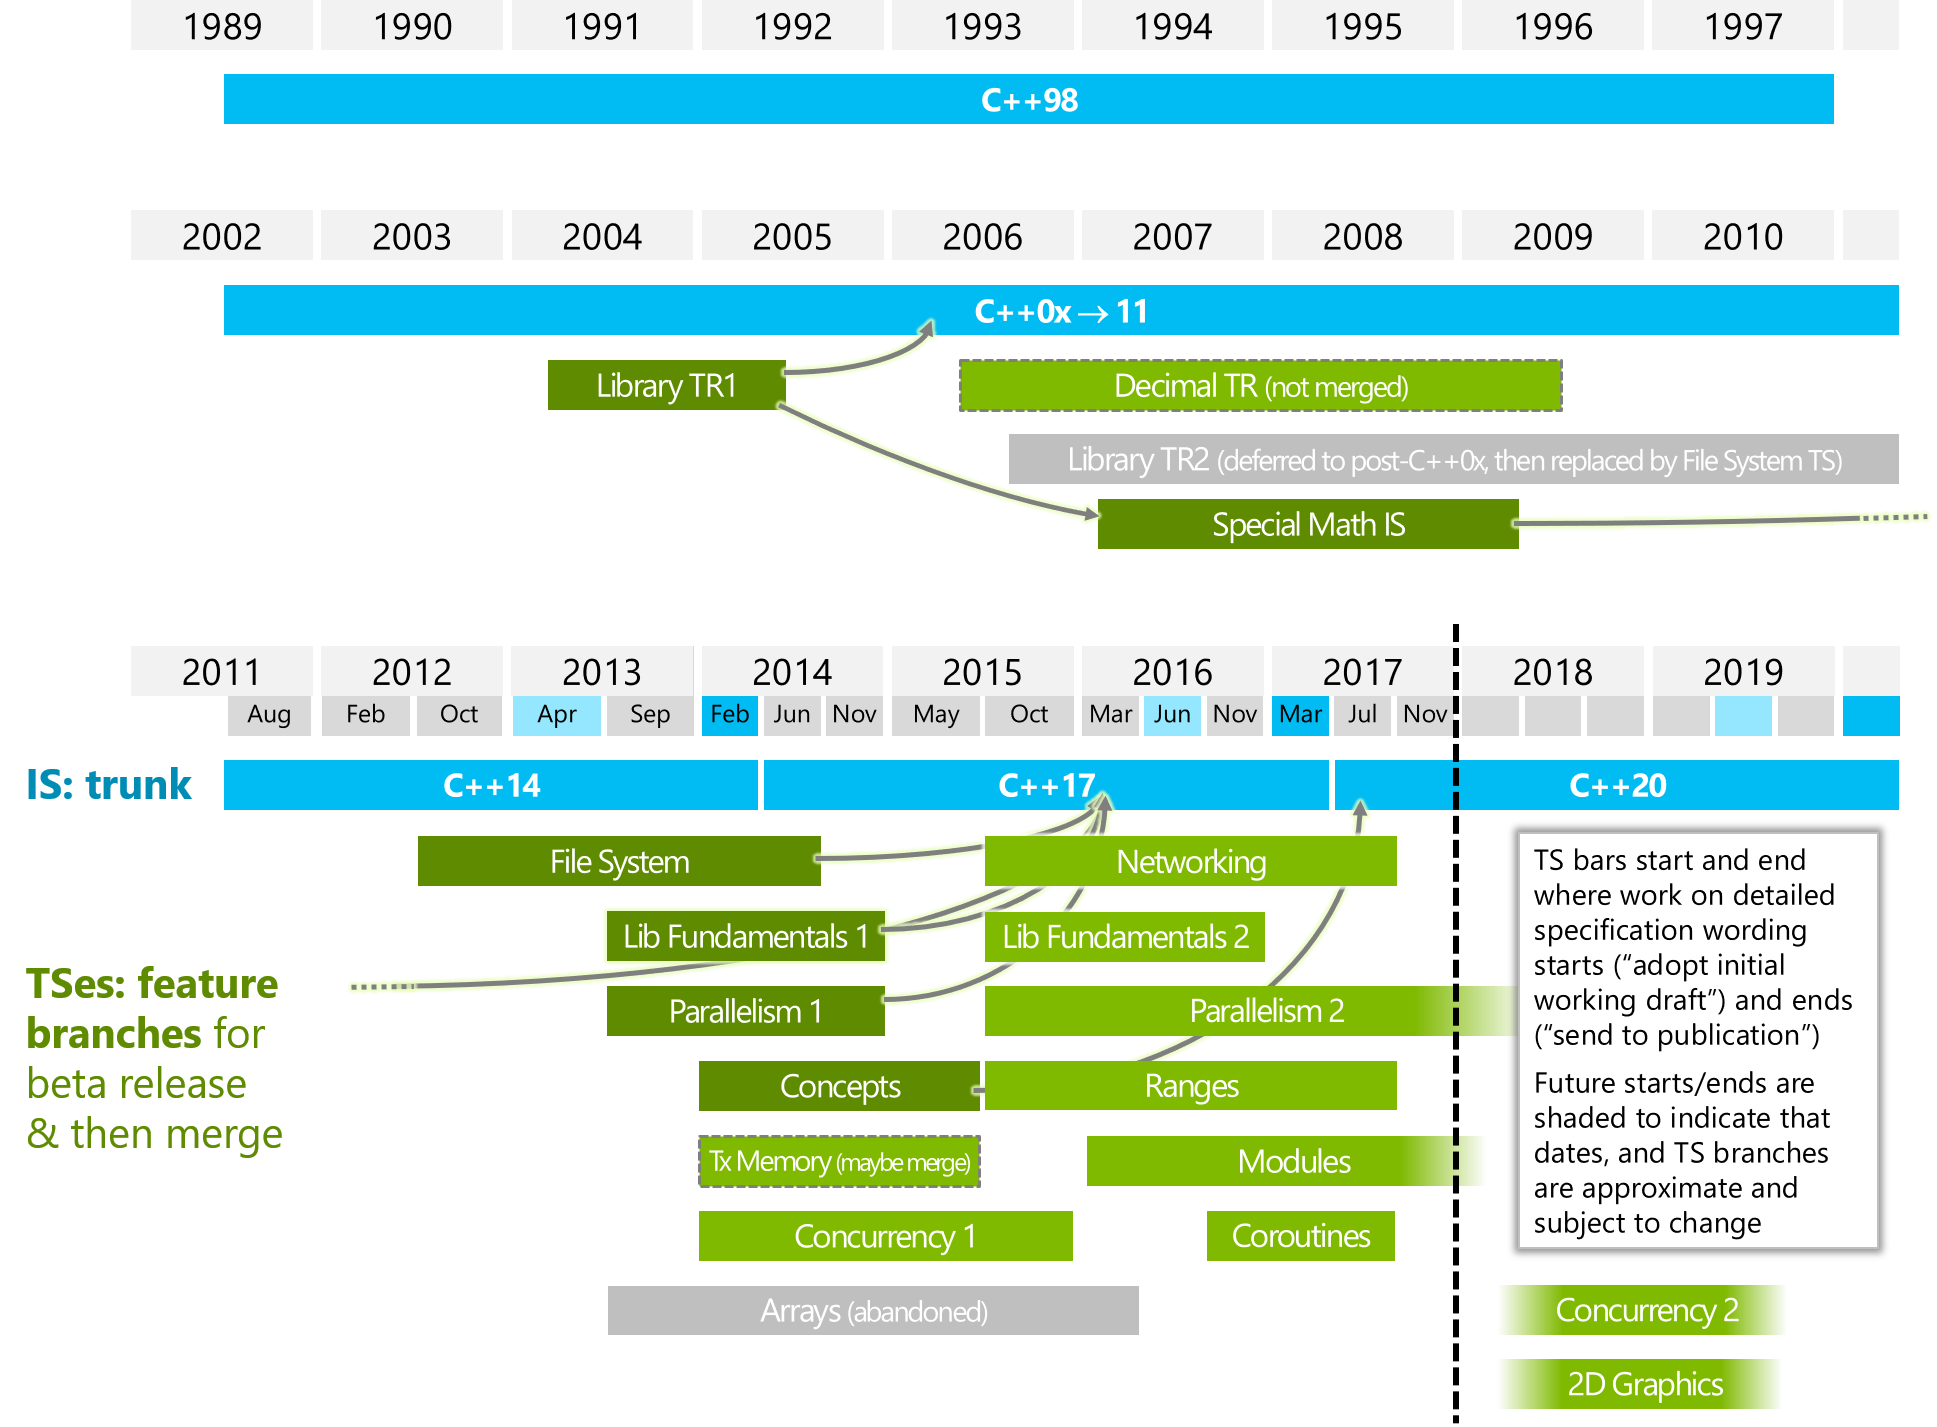
\includegraphics[width=\textwidth]{img/wg21-timeline.png}
\end{frame}

\begin{frame}[t]{Evolución}
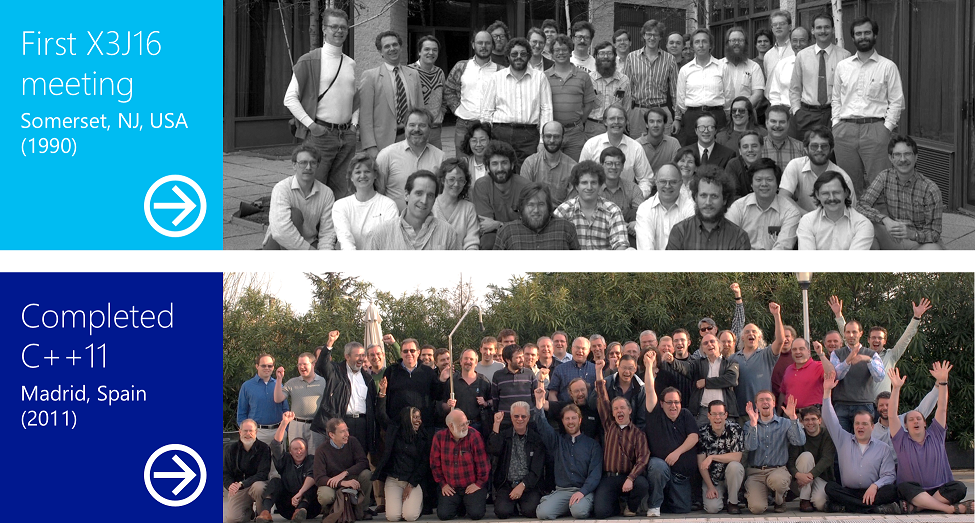
\includegraphics[width=\textwidth]{img/wg21-1990-2011.png}
\end{frame}

\begin{frame}[t]{C++14}

\includegraphics[width=\textwidth]{img/cpp-14.jpg}
\end{frame}

\begin{frame}[t]{C++17}

\includegraphics[width=\textwidth]{img/cpp-17.jpg}
\end{frame}


\section{Pequeños cambios}

\subsection{Trigrafos}

\begin{frame}[t]{Adios a los trigrafos}
\begin{itemize}
  \item Un \textmark{trigrafo} es una secuencia de caracteres que permite \emph{simular}
        otro carácter.
    \begin{itemize}
      \item Ejemplos:
        \begin{itemize}
          \item \cppid{??=} \quad $\Rightarrow$ \quad \cppid{\#}.
          \item \cppid{??-} \quad $\Rightarrow$ \quad \cppid{\~}.
          \item \ldots
        \end{itemize}
    \end{itemize}

  \vfill\pause
  \item En C++17 los \textmark{trigrafos} \textbad{dejan de ser estándar}.
    \begin{itemize}
      \item Limitada utilidad hoy en día.
      \item Simplifica el análisis de código.
    \end{itemize}
\end{itemize}
\end{frame}

\subsection{Keyword \bf{\texttt{register}}}

\begin{frame}[t,fragile]{¡Hasta luego \textbf{register}!}
\begin{itemize}
  \item La palabra reservada \cppkey{register} está \textmark{despreciada}
        desde C++11.
\begin{block}{Uso legado de \textbf{register}}
\begin{lstlisting}
for (register int i=0; i<10; ++i) {
  v[i] = w[i];
}
\end{lstlisting}
\end{block}
  \vfill
  \item \textmark{Eliminado} en C++17.
  \vfill
  \item La palabra \cppkey{register} se mantiene \textmark{reservada}
        para uso futuro.
\end{itemize}
\end{frame}

\subsection{Incremento de booleanos}

\begin{frame}[t,fragile]{Eliminando \textbf{\texttt{operator++(bool)}}}
\begin{itemize}
  \item El operador \cppkey{++} sobre valores \cppkey{bool} ha estado
        \textmark{despreciado} desde C++98.
\vfill
\begin{block}{Usando el operador ++}
\begin{lstlisting}
bool x = false;
x++; // x == true
x++; // x == true
if (x++) do_whatever();
if (std::exchange(x,true)) do_whatever();
\end{lstlisting}
\end{block}
\vfill
  \item Se elimina de C++17
\end{itemize}
\end{frame}

\subsection{Especificaciones dinámicas de excepciones}

\begin{frame}[t,fragile]{Especifando excepciones}
\begin{itemize}
  \item Las especificaciones dinámicas de excepciones están \textmark{despreciadas}
        desde C++11.
\vfill
\begin{block}{Especificaciones de excepciones}
\begin{lstlisting}
void f() throw (std::logic_error);
void g() throw();
\end{lstlisting}
\end{block}
  \vfill\pause
  \item Se eliminan en C++17
\begin{block}{Especificaciones de excepciones}
\begin{lstlisting}
void f();
void g() noexcept;
\end{lstlisting}
\end{block}
\end{itemize}
\end{frame}

\subsection{Clase \bf\texttt{auto\_ptr}}

\begin{frame}[t]{Punteros inteligentes}
\begin{itemize}
  \item \textgood{C++11} incorporó nuevos \textmark{punteros inteligentes}:
    \begin{itemize}
      \item \cppid{unique\_ptr}.
      \item \cppid{shared\_ptr}.
      \item \cppid{weak\_ptr}.
    \end{itemize}

  \vfill
  \item \textgood{C++11} despreció un \textmark{puntero inteligente}:
    \begin{itemize}
      \item \cppid{auto\_ptr}.
    \end{itemize}

  \vfill\pause
  \item \textgood{C++17} \textbad{elimina} \cppid{auto\_ptr}.
\end{itemize}
\end{frame}

\subsection{Reglas para iniciación y auto}

\begin{frame}[t,fragile]{Iniciación de lista}
\begin{itemize}
  \item C++11 introdujo la \textgood{iniciación uniforme} y \cppkey{auto}.
  \vfill\pause
  \item Dos tipos de iniciación:
    \begin{itemize}
      \item \textenum{Iniciación de copia}:
\begin{lstlisting}
auto x = {a, b, c}; // x es initializer_list<decltype(a)>
auto y = {a};       // y es initializer_list<decltype(a)> 
\end{lstlisting}
      \item \textenum{Iniciación directa}:
\begin{lstlisting}
auto x {a, b, c}; // x es initializer_list<decltype(a)>
auto y {a};       // y es initializer_list<decltype(a)>, pero confuso
\end{lstlisting}
    \end{itemize}
  \vfill\pause
  \item C++17 resuelve la confusión
\begin{lstlisting}
auto x {a, b, c}; // x es initializer_list<decltype(a)>
auto y {a};       // y es decltype(a)
\end{lstlisting}
\end{itemize}
\end{frame}  

\subsection{\bf{\texttt{static\_assert}}}

\begin{frame}[t,fragile]{Aserciones en tiempo de compiación}
\begin{itemize}
  \item C++11 introdujo las aserciones en tiempo de compilación.
\begin{lstlisting}
template <typename T>
void f(T & x) {
  static_assert(std::is_integral_v<T>, 
      "T debe ser un tipo numérico integral");
  //...
}

void g() {
  f(5); // OK
  f(1.0); // Error de compilación
  // ...
}
\end{lstlisting}

  \vfill\pause
  \item C++17 hace el mensaje opcional.
    \begin{itemize}
      \item En muchos casos el mensaje por defecto es suficiente.
      \item Evita tener que replicar el texto dos veces.
    \end{itemize}
\end{itemize}
\end{frame}


\section{Aclaraciones}

\subsection{Orden de evaluación}

\begin{frame}[t,fragile]{Orden de evaluación}
\begin{itemize}
  \item Orden de evaluación de operandos en C++11:
\begin{lstlisting}[basicstyle=\scriptsize]
void f() {
  std::string s = "but I have heard it works even if you don't believe in it";
  s.replace(0, 4, "").replace(s.find("even"), 4, "only").replace(
      s.find(" don't"), 6, "");
  assert(s == "I have heard it works only if you believe in it");
  //...
}
\end{lstlisting}

  \vfill\pause
  \item \textmark{Problema}:
    \begin{itemize}
      \item Encadenamiento de llamadas a funciones miembro.
      \item Orden ejecución no definido en C++11.
      \item Error en \emph{``The C++ Programming Language. 4 Ed.''}.
    \end{itemize}
\end{itemize}
\end{frame}

\begin{frame}[t,fragile]{Orden de evaluación}
\begin{itemize}
  \item Otro ejemplo en C++11:
\begin{lstlisting}
void f() {
  std::map<int,int> v;
  v[0] = v.size();
  //...
}
\end{lstlisting}
  \item \textmark{Resultado}:
    \begin{itemize}
      \item \cppid{\{0,0\}}.
      \item \cppid{\{0,1\}}.
    \end{itemize}
\end{itemize}
\end{frame}

\begin{frame}[t,fragile]{Fijando el orden en C++17}
\begin{itemize}
  \item Se fija el orden de evaluación en:
    \begin{itemize}
      \item \cppid{a.b}
      \item \cppid{a->b}
      \item \cppid{a->*b}
      \item \cppid{a(b1,b2,b3)}
      \item \cppid{b op= a}
      \item \cppid{a[b]}
      \item \cppid{a << b}
      \item \cppid{a >> b}
    \end{itemize}

  \vfill\pause
  \item Pero:
    \begin{itemize}
      \item No se define el orden de evaluación de argumentos de función.
    \end{itemize}
\end{itemize}
\end{frame}

\subsection{Elusión de copia}

\begin{frame}[t]{Eludiendo copias temporales}
\begin{itemize}
  \item El estándar C++11 \textmark{permite evitar} copias intermedias en algunos casos:
    \begin{itemize}
      \item Cuando se inicia un objeto con otro objeto temporal.
      \item Cuando se devuelve una variable local.
      \item Cuando se captura una excepción por valor.
    \end{itemize}
  \vfill\pause
  \item Pero:
    \begin{itemize}
      \item Es una optimización opcional.
      \item Hace falta definir constructores de copia por si el compilador no optimiza.
      \item C++17 asegura la optimización
    \end{itemize}
\end{itemize}
\end{frame}

\begin{frame}[t,fragile]{Ejemplo de elusión}
\begin{lstlisting}
class X {
public:
  X(int n);
  X(const X &) = delete;
  X(X &&) = delete;
  //...
};

X make_x(int z) { return X{z}; }

void f() {
  auto a = make_x(10); // Portable desde C++17
}
\end{lstlisting}
\end{frame}

\subsection{Excepciones y punteros a función}

\begin{frame}[t,fragile]{Especificaciones de excepción}
\begin{itemize}
  \item Las especificaciones de excepciones pasan a formar parte
        del tipo de la función.
\begin{lstlisting}
  // p1_t y p2_t son dos tipos distintos
  using p1_t = int(*)(char) noexcept;
  using p2_t = int(*)(char);
\end{lstlisting}
\vfill\pause
  \item Se puede convertir un valor de tipo puntero a excepción \cppkey{noexcept},
        a un tipo puntero a excepción.
\begin{lstlisting}
  int f(char);
  int g(char) noexcept;
  //...
  p1_t p1f = f; // Error 
  p1_t p1g = g; // OK 
  p2_t p2f = f; // OK
  p2_t p2g = g; // Conversión
\end{lstlisting}
\end{itemize}
\end{frame}

\subsection{Memoria dinámica sobre-alineada}

\begin{frame}[t,fragile]{\bf\texttt{new} y alineamiento}
\begin{itemize}
  \item En C++11/14 no hay garantías de alineamiento con \cppkey{new}.
\begin{lstlisting}
struct alignas(16) vec {
  float val[4];
};

float * v = new vec[100];
\end{lstlisting}

  \vfill\pause
  \item C++17 tiene en cuenta el alineamiento.
\begin{lstlisting}
void* operator new(size_t, align_val_t);
void* operator new[](size_t, align_val_t);
void operator delete(void*, align_val_t);
void operator delete[](void*, align_val_t);
void operator delete(void*, size_t, align_val_t);
void operator delete[](void*, size_t, align_val_t);
\end{lstlisting}

\end{itemize}
\end{frame}


\section{Programación genérica}

\subsection{Deducción de argumentos de plantilla de clase}

\begin{frame}[t,fragile]{Deducción de argumentos de función}
\begin{itemize}
  \item En C++ siempre se deducen argumentos de plantilla implícitamente.
\begin{lstlisting}
template <typename T>
void f(T & x);

void g() {
  f(2); // f<int>(2)
  f(1.0); // f<double>(1.0)
   
  complex<float> z;
  f(z);  // f<complex<float>>(z);

  vector<map<int,string>> v;
  f(v); // f<vector<map<int,string>>>
}
\end{lstlisting}
\end{itemize}
\end{frame}

\begin{frame}[t,fragile]{Deduccion de argumentos de clase}
\begin{itemize}
  \item Sin embargo, para clases \ldots
\begin{lstlisting}
void g() {
  std::pair<int,string> p{1969, "Daniel"};

  auto q = std::make_pair(1950, "Bjarne");

  std::pair r{1955, "James"}; // Error faltan argumentos de plantilla
}
\end{lstlisting}

  \vfill
  \item No se pueden deducir los argumentos de plantilla en constructor.

\end{itemize}
\end{frame}

\begin{frame}[t,fragile]{Deducción de argumentos}
\begin{itemize}
  \item En C++17 se pueden deducir los argumentos de plantilla de clase.
\begin{lstlisting}
std::pair p{1969, "Daniel"s}; // std::pair<int,std::string>

std::map<int,double> create_dic();
// std::tuple<int, double, std::map<int,double>>
std::tuple q{1, 2.5, create_dic()};
\end{lstlisting}
\end{itemize}
\end{frame}

\begin{frame}[t,fragile]{Simplificación de código}
\begin{itemize}
  \item Sin deducción:
\begin{lstlisting}
std::mutex m1;
std::recursive_mutex m2;
std::shared_lock<std::recursive_mutex> sl{m2};
std::lock_guard<std::mutex, std::shared_lock<std::recursive_mutex>> l{m1,s1};
\end{lstlisting}

  \vfill\pause
  \item Con deducción en C++17:
\begin{lstlisting}
std::mutex m1;
std::recursive_mutex m2;
std::shared_lock sl{m2};
std::lock_guard l{m1,s1};
\end{lstlisting}

\end{itemize}
\end{frame}

\subsection{Deducción de valores en plantillas}

\begin{frame}[t,fragile]{Valores como argumentos de plantilla}
\begin{itemize}
  \item Un argumento de plantilla puede ser un valor.
\begin{lstlisting}
template <int n>
class table;

table<10> t1; // n==10
table<100> t2; // n==100
\end{lstlisting}

  \vfill\pause
  \item Se puede generalizar el tipo del valor
\begin{lstlisting}
template <typename T, T n>
class table;

table<10> t1; // table<int,10>
table<100UL> t2; // table<unsigned long, 100UL>
\end{lstlisting}

\end{itemize}
\end{frame}

\begin{frame}[t,fragile]{Simplificando argumentos valor}
\begin{itemize}
  \item Se puede usar \cppkey{auto}:
\begin{lstlisting}
template <auto n>
class table;

table<10> t1; // decltype(n)=int, n=10
table<100UL> t2; // decletype(n)=unsigned long, n=100UL
\end{lstlisting}
\end{itemize}
\end{frame}


\subsection{Plegamiento de expresiones}

\begin{frame}[t,fragile]{Sumando varios valores}
\begin{itemize}
  \item Una función genérica de suma:
\begin{lstlisting}
auto suma() { return 0; }

template <typename T1>
auto suma(T1 v1) { return v1; }

template <typename T1, typename T2>
auto suma(T1 v1, T2 v2) { return v1+v2; }

template <typename T1, typename T2, typename T3>
auto suma(T1 v1, T2 v2, T3 v3) { return v1+v2+v3; }

//...

void f() {
  auto x = suma(1, 2.0);
  auto y = suma(1L, 1.5f, 2LL);
  //...
}
\end{lstlisting}
\end{itemize}
\end{frame}

\begin{frame}[t,fragile]{Suma variádica}
\begin{itemize}
  \item Una función genérica de suma en C++11:
\begin{lstlisting}
auto suma() { return 0; }

template <typename T1, typename ... Ts>
auto suma(T1 x1, Ts ... xs) {
  return x1 + suma(xs...);
}

void f() {
  auto x = suma(1, 2.0);
  auto y = suma(1L, 1.5f, 2LL);
  //...
}
\end{lstlisting}
\end{itemize}
\end{frame}

\begin{frame}[t,fragile]{Plegando expresiones}
\begin{itemize}
  \item En C++17 se puede aplicar plegamiento para algunos operadores.
\begin{lstlisting}
template <typename ... Ts>
auto suma(Ts ... xs) { return (xs + ... + 0); }
\end{lstlisting}
  \vfill
  \item o bien:
\begin{lstlisting}
template <typename ... Ts>
auto suma(Ts ... xs) { return (... + xs); }
\end{lstlisting}

  \vfill\pause
  \item Expresiones válidas:
    \begin{itemize}
      \item \cppid{(\ldots $\otimes$ args)} \quad $\rightarrow$ \quad 
            $(\ldots((a_1 \otimes a_2) \otimes a_3) \otimes \ldots) \otimes a_n$
      \item \cppid{(x $\otimes$ \ldots $\otimes$ args)} \quad $\rightarrow$ \quad
            $(\ldots((x \otimes a_1) \otimes a_2) \otimes \ldots) \otimes a_n$
      \item \cppid{(args $\otimes$ \ldots)} \quad $\rightarrow$ \quad
            $a_1 \otimes (\ldots \otimes (a_{n-1} \otimes a_n))$ 
      \item \cppid{(args $\otimes$ \ldots $\otimes$ x)} \quad $\rightarrow$ \quad
            $a_1 \otimes (\ldots \otimes (a_{n-1} \otimes (a_n \otimes x)))$ 
    \end{itemize}
\end{itemize}
\end{frame}

\subsection{{\bf if} en tiempo de compilación}

\begin{frame}[t,fragile]{SFINAE}
\begin{itemize}
  \item Dos versiones de una función con SFINAE.
\begin{lstlisting}
template <typename T,
          std::enable_if_t<std::is_pointer<T>::value> * = nullptr>
auto get(T v) { return *v; }

template <typename T,
          std::enable_if_t<!std::is_pointer<T>::value> * = nullptr>
auto get(T v) { return v; }

void f() {
  int x;
  int * p = x;

  auto z1 = get(x);
  auto z2 = get(p);
}
\end{lstlisting}
\end{itemize}
\end{frame}

\begin{frame}[t,fragile]{Tag dispatching}
\begin{itemize}
  \item Dos versiones con \emph{tag dispatching}.
\begin{lstlisting}
template <typename T>
auto get(T v, std::true_type) { return * v; }

template <typename T>
auto get(T v, std::false_type) { return v; }

template <typename T>
auto get(T v) { return get(t, std::is_pointer<T>::value); }

void f() {
  int x;
  int * p = x;

  auto z1 = get(x);
  auto z2 = get(p);
}
\end{lstlisting}
\end{itemize}
\end{frame}

\begin{frame}[t,fragile]{Selección en tiempo de compilación}
\begin{itemize}
  \item Se pueden usar sentencias \cppid{if} que se evalúan en tiempo de compilación.
\begin{lstlisting}
template <typename T>
auto get(T v) { 
  if constexpr (std::is_pointer_v<T>) { return *v; }
  else { return v; }
}

void f() {
  int x;
  int * p = x;

  auto z1 = get(x);
  auto z2 = get(p);
}
\end{lstlisting}
\end{itemize}
\end{frame}

\subsection{Otros cambios en programación genérica}

\begin{frame}[t]{Más sobre plantillas}
\begin{itemize}
  \item Uso de \cppkey{typename} en vez de \cppkey{class} en parámetros
        plantilla de plantilla (\emph{template template parameters}).
  \item Mejora de compatibilidad plantilla de plantillas con parámetros por defecto.
  \item Menos restricciones para parámetros de plantilla que no son tipos.
    \begin{itemize}
      \item Punteros, referencias, y punteros a miembro.
    \end{itemize}
  \item Posibilidad de definir expresiones lambda que son \cppkey{constexpr}.
\end{itemize}
\end{frame}


\section{Atributos}

\subsection{Atributos en C++11/14}

\begin{frame}[t,fragile]{Atributos}
\begin{itemize}
  \item Una manera portable de introducir anotaciones.
    \begin{itemize}
      \item Mejor que \cppkey{\_\_attribute\_\_}, \cppkey{\_\_declspec}, \ldots
      \item No pueden tener efecto semántico.
    \end{itemize}
  \vfill\pause
  \item Atributos existentes en C++11:
    \begin{itemize}
      \item \cppid{[[noreturn]]}.
      \item \cppid{[[carries\_dependency]]}.
      \item \cppkey{alignas}\cppid{(num)}.
    \end{itemize}
  \vfill\pause
  \item Atributos añadidos en C++14:
    \begin{itemize}
      \item \cppid{[[deprecated]]}.
      \item \cppid{[[deprecated("mensaje")]]}.
    \end{itemize}
\end{itemize}
\end{frame}

\subsection{Nuevos atributos}

\begin{frame}[t,fragile]{Sentencias {\bf switch}}
\begin{itemize}
  \item Errores típicos en sentencias \cppkey{switch}:
\begin{lstlisting}
switch (estado) {
  case modo::inicio:
    procesa_inicio(); // ¿Paso intencionado a siguiente caso?
  case modo::intermedio:
    procesa_intermedio();
    break;
  case modo::fin:
    procesa_fin(); // ¿Paso intencionado a siguiente caso?
  default:
    procesa_defecto();
}
\end{lstlisting}
\end{itemize}
\end{frame}

\begin{frame}[t,fragile]{Mejorando {\bf switch}}
\begin{itemize}
  \item Fuerza a ser explícito sobre la intención con atributo \cppid{[[fallthrough]]}.
\begin{lstlisting}
switch (estado) {
  case modo::inicio:
    procesa_inicio(); // Warning: fallthrough implícito
  case modo::intermedio:
    procesa_intermedio();
    break;
  case modo::fin:
    procesa_fin(); // OK: falltrhough explícito
    [[fallthrough]];
  default:
    procesa_defecto();
}
\end{lstlisting}
\end{itemize}
\end{frame}

\begin{frame}[t,fragile]{Ignorando resultados}
\begin{itemize}
  \item C++ permite ignorar el resultado de una función:
\begin{lstlisting}
int lee_bytes(std::ifstream & f, int n);
//...
void f(std::ifstream & fs) {
  lee_bytes(fs, 100); // resultado ignorado
  //...
}
\end{lstlisting}

  \vfill\pause
  \item Se pude forzar que no se pueda ignorar con \cppkey{[[nodiscard]]}:
\begin{lstlisting}
[[nodiscard]] int lee_bytes(std::ifstream & f, int n);
//...
void f(std::ifstream & fs) {
  lee_bytes(fs, 100); // warning: resultado ignorado
  int r = lee_bytes(fs, 50); // OK
  //...
}
\end{lstlisting}

\end{itemize}
\end{frame}

\begin{frame}[t,fragile]{Tipos no descartables}
\begin{itemize}
  \item Se puede marcar un tipo como \textmark{no descartable}:
\begin{lstlisting}
[[nodiscard]] struct resultado {
  int resultado;
  string mensaje;
};

resultado haz_algo();

void f() {
  haz_algo(); // warning: resultado descartado
  auto r = haz_algo(); // OK
  //...
}
\end{lstlisting}
\end{itemize}
\end{frame}

\begin{frame}[t,fragile]{Variables no usadas}
\begin{itemize}
  \item La mayoría de los compiladores emiten una advertencia si no 
        se usa una variable.
\begin{lstlisting}
void f(int a, int b) { // warning: b no usado
  int z = 0; // warning: z no usado 
  return a *2;
}
\end{lstlisting}

  \vfill\pause
  \item Se puede expresar la intención con \cppkey{[[maybe\_unused]]}:
\begin{lstlisting}
void f(int a, [[maybe_unused]] int b) { // OK: b no usado
  [[maybe_unused]] int z = 0; // OK: z no usado 
  return a *2;
}
\end{lstlisting}
\end{itemize}
\end{frame}

\subsection{Otras modificaciones sobre atributos}

\begin{frame}[t,fragile]{Atributos en nuevos lugares}
\begin{itemize}
  \item Se añaden atributos a nuevos elementos:
    \begin{itemize}
      \item Espacios de nombre:
\begin{lstlisting}
namespace [[deprecated]] mi_lib_anterior {
  void f1();
  //...
}

void g() {
  mi_lib_anterior::f1(); // Warning: deprecated
  //...
}
\end{lstlisting}

      \item Enumeradores de un enumerado:
\begin{lstlisting}
enum modo {
  apagado,
  encendiendo [[deprecated]],
  encendido
};	
\end{lstlisting}
    \end{itemize}
\end{itemize}
\end{frame}

\begin{frame}[t,fragile]{Atributos desconocidos ignorados}
\begin{itemize}
  \item Antes de C++17 un compilador podía dar un error para un atributo
        que no reconocía (p.ej. de otro compilador):
\begin{lstlisting}
void f(void * p) {
  [[gsl::supress("type")]]  // Solamente reconocido por clang-tidy
  int * q = reinterpret_cast<int*>(p);
  //...
}
\end{lstlisting}
  \vfill
  \item Ahora no puede dar un error.
    \begin{itemize}
      \item Aunque si un warning.
    \end{itemize}
\end{itemize}
\end{frame}

\begin{frame}[t,fragile]{Espacios de nombre y atributos}
\begin{itemize}
  \item En C++11/14 los espacios de nombre de atributos deben cualificar
        explícitamente cada atributo.
\begin{lstlisting}
void f(X x, Y y) {
  [[rpr::kernel, rpr::target(cpu,gpu,fpga), rpr::in(x), rpr::out(y)]]
  do_f(x,y);
  //...
}
\end{lstlisting}

  \vfill\pause
  \item En C++17 se puede evitar la repetición:
\begin{lstlisting}
void f(X x, Y y) {
  [[using rpr: kernel, target(cpu,gpu,fpga), in(x), out(y)]]
  do_f(x,y);
  //...
}
\end{lstlisting}

\end{itemize}
\end{frame}


\section{Simplificaciones}

\subsection{Vinculación estructurada}

\begin{frame}[t,fragile]{Múltiples valores de retorno}
\begin{itemize}
  \item En C++14, se pueden gestionar múltiples valores de retorno con
        \cppid{std::tuple} y \cppid{std::tie}.
\begin{lstlisting}
std::tuple<int, string, bool> f() {
  return make_tuple(1, "hola", false);
}

void g() {
  int n;
  std::string msg;
  bool result;
 
  std::tie(n, msg, result) = f();
  //...
}
\end{lstlisting}
\end{itemize}
\end{frame}

\begin{frame}[t,fragile]{Vinculación estructurada}
\begin{itemize}
  \item En C++17, se introducen las \textmark{vinculaciones estructuradas}:
\begin{lstlisting}
std::tuple<int, string, bool> f() {
  return make_tuple(1, "hola", false);
}

void g() {
  auto [n, msg, result] = f();
  //...
}
\end{lstlisting}
\end{itemize}
\end{frame}

\begin{frame}[t,fragile]{Otras vinculaciones estructuradas}
\begin{itemize}
  \item Las vinculaciones estructuradas no están limitadas a tuplas.
    \begin{itemize}
      \item Arrays:
\begin{lstlisting}
double v[] = {1, 2, 3};
auto [a,b,c] = v;
\end{lstlisting}

      \vfill\pause
      \item Para cualquier tipo que soporte \cppid{tuple\_size<>} y \cppid{get<N>()}
            (p. ej. \cppid{std::pair}).
\begin{lstlisting}
pair<int,string> f();

auto [x,y] = f();
\end{lstlisting}

      \vfill\pause
      \item Estructuras sin datos miembro estáticos.
\begin{lstlisting}
struct X { int a; double b; char c; };
X f();
const auto [x,y,z] = f();
\end{lstlisting}
    \end{itemize}
\end{itemize}
\end{frame}

\begin{frame}[t,fragile]{Combinando vinculaciones estructuradas y bucles de rango}
\begin{itemize}
  \item Se pueden combinar las vinculaciones estructuradas con el uso
        de bucles for basados en rango.
\begin{lstlisting}
std::map<int, std::string> dic;
//...
for (auto & [id, nombre] : dic) {
  cout << "Id: " << id << "\n";
  cout << "Nombre: " << nombre << "\n";
}
\end{lstlisting}
\end{itemize}
\end{frame}

\subsection{Iniciación en {\bf if} y {\bf switch}}

\begin{frame}[t,fragile]{Iniciación en \textbf{if}}
\begin{itemize}
  \item Se extiende la sintaxis de \cppkey{if} para introducir declaraciones de variable.
\begin{lstlisting}
if (init; cond) statement;
\end{lstlisting}
\end{itemize}

\vfill\pause
\begin{columns}[T]

\column{.5\textwidth}
\begin{block}{Antes}
\begin{lstlisting}
{
  auto val = get_value();
  if (val>0) {
    f(val);
  }
  else throw invalid{}; 
}
\end{lstlisting}
\end{block}

\pause
\column{.5\textwidth}
\begin{block}{Después}
\begin{lstlisting}
if (auto val = get_value(); val>0) {
  f(val);
}
else throw invalid{};
\end{lstlisting}
\end{block}

\end{columns}
\end{frame}


\begin{frame}[t,fragile]{Buscando en cadenas}
\begin{block}{Antes}
\begin{lstlisting}
{
  const auto it = texto.find("hola");
  if (it != string::npos) {
    cout << "Encontrado en posición "
      << distance(text.begin(), it) << "\n"
  }
}
\end{lstlisting}
\end{block}

\pause
\begin{block}{Después}
\begin{lstlisting}
if (const auto it = texto.find("hola"); it != string::npos) {
  cout << "Encontrado en posición "
    << distance(text.begin(), it) << "\n"
}
\end{lstlisting}
\end{block}
\end{frame}

\begin{frame}[t,fragile]{Buscando en un mapa}
\begin{itemize}
  \item Se puede combinar con vinculaciones estructuradas.
\end{itemize}
\begin{lstlisting}
std::map<int,std::string> m;
//...
if (auto & [it, encontrado] : m.insert(valor); encontrado) {
  f(it);
}
\end{lstlisting}
\end{frame}

\begin{frame}[t,fragile]{Iniciación en \textbf{switch}}
\begin{itemize}
  \item Funcionalidad extendida también a \cppkey{switch}:
\end{itemize}
\begin{lstlisting}
switch (auto x = get_value(); x.status()) {
  case abierto:
    procesa_abierto(x);
    break;
  case cerrado:
    procesa_cerrado(x);
    break;
}
\end{lstlisting}
\end{frame}

\subsection{Variables inline}

\begin{frame}[t]{Variables \textbf{inline}}
\begin{itemize}
  \item Una variable marcada como \cppkey{inline}:
    \begin{itemize}
      \item Puede aparecer en varias unidades de traducción si tiene
            la misma definición.
        \begin{itemize}
          \pause
          \item Permite poner la definición en un archivo de cabecera.
        \end{itemize}
      \pause
      \item Debe estar definida en cada unidad de traducción en la que
            se usa.
      \pause
      \item Hay una única instancia.
    \end{itemize}

  \vfill\pause
  \item Los datos miembro que sean \cppkey{constexpr} y \cppkey{static} son
        implícitamente \cppkey{inline}.
\end{itemize}
\end{frame}

\begin{frame}[t,fragile]{Constantes en C++14}
\begin{columns}[T]

\column{.5\textwidth}

\begin{block}{tabla.h}
\begin{lstlisting}
static constexpr max_elem = 4096;

class tabla {
  //...
private:
  static constexpr max_valor = 1000000;
  //...
};
\end{lstlisting}
\end{block}

\column{.5\textwidth}
\begin{block}{tabla.cpp}
\begin{lstlisting}
static constexpr max_elem;
static constexpr tabla::max_valor;
\end{lstlisting}
\end{block}

\end{columns}
\end{frame}


\begin{frame}[t,fragile]{Constantes en C++17}
\begin{columns}[T]

\column{.5\textwidth}

\begin{block}{tabla.h}
\begin{lstlisting}
inline static constexpr max_elem = 4096;

class tabla {
  //...
private:
  // Implícitamente inline
  static constexpr max_valor = 1000000;
  //...
};
\end{lstlisting}
\end{block}

\column{.5\textwidth}
\begin{block}{tabla.cpp}
\begin{lstlisting}
// Sin definiciones de constantes
// ...
\end{lstlisting}
\end{block}
 
\end{columns}
\end{frame}




\section{Algoritmos paralelos}

\subsection{Políticas de ejecución}

\begin{frame}[t]{Introducción}
\begin{itemize}
  \item Una \textbf{Política de ejecución} indica el tipo de paralelismo
        que se permite en la ejecución de un algoritmo.
    \begin{itemize}
      \item \textbf{Secuencial}: Sin paralelizar.
        \begin{itemize}
          \item Tipo: \cppid{std::execution::sequenced\_policy}
          \item Objeto global: \cppid{std::execution::seq}.
        \end{itemize}
      \item \textbf{Paralelo}: Paralelizado.
        \begin{itemize}
          \item Tipo: \cppid{std::execution::parallel\_policy}.
          \item Objeto global: \cppid{std::execution::par}.
        \end{itemize}
      \item \textbf{Paralelo + Vector}: Paralelizado y vectorizado.
        \begin{itemize}
          \item Tipo: \cppid{std::execution::parallel\_unsequenced\_policy}.
          \item Objeto global: \cppid{std::execution::par\_unseq}.
        \end{itemize}
    \end{itemize}
\end{itemize}
\end{frame}

\begin{frame}[t,fragile]{Versiones de algoritmos}
\begin{itemize}
  \item Todos los algoritmos paralelos toman como primer parámetro una política
        de ejecución.
\end{itemize}
\begin{block}{Ejemplo: ordenando un vector}
\begin{lstlisting}
using namespace std;
vector<double> v = read_values();
sort(v.begin(), v.end());

using namespace std::execution;

sort(seq, v.begin(), v.end()); // Secuencial
sort(par, v.begin(), v.end()); // Paralelo
sort(par_unseq, v.begin(), v.end()); // Paralelo+Vect
\end{lstlisting}
\end{block}
\end{frame}


\subsection{Visión general}

\begin{frame}[t]{¿Qué algoritmos se incluyen?}
\begin{itemize}
  \item La biblioteca de algoritmos paralelos incluye la mayor parte
        de los algoritmos de la STL.
  \item En todos los casos se añade un parámetro adicional para indicar
        la política de ejecución.
    \begin{itemize}
      \item Este parámetro se coloca el primero.
    \end{itemize}
  \item Hay algoritmos de la STL que pueden no estar.
    \begin{itemize}
      \item Ejemplo \cppid{accumulate}.
    \end{itemize}
  \item Hay algoritmos que no provienen de la STL.
    \begin{itemize}
      \item Ejemplo: \cppid{exclusive\_scan}
    \end{itemize}
\end{itemize}
\end{frame}

\begin{frame}[t,fragile]{Buscando en una secuencia}
\begin{block}{Ejemplos}
\begin{lstlisting}g
vector<int> v = get_values_vector();
count_if(par, begin(v), end(v), 
  [](int x) { return x>0; });
auto p = find(par, begin(v), end(v), 0);
auto q = find_if(par, begin(v), end(v),
  [](int x) { return (x>0) && (x<10); }
\end{lstlisting}
\end{block}
\end{frame}


\subsection{Algoritmos no numéricos}

\begin{frame}[t]{Algoritmos no numéricos}
\begin{itemize}
  \item Son algoritmos que no requieren que los valores accedidos por
        los iteradores sean de un tipo numérico.
    \begin{itemize}
      \item Más generales que los algoritmos numéricos.
    \end{itemize}
  \item Ejemplos:
    \begin{itemize}
      \item \cppid{for\_each()}.
      \item \cppid{for\_each\_n()}.
    \end{itemize}
\end{itemize}
\end{frame}

\begin{frame}[t,fragile]{For Each}
\begin{lstlisting}g
template <class ExecutionPolicy, class InputIterator, class Function>
void for_each(ExecutionPolicy && ep, 
              InputIterator first, InputIterator last,
              Function f);
\end{lstlisting}
\begin{itemize}
  \item Aplica \cppid{f} al resultado de desreferenciar cada iterador en el rango \cppid{[first,last)}.
\end{itemize}
\begin{block}{Ejemplo}
\begin{lstlisting}g
long cuenta_primos(const vector<int> & v) {
  std::atomic<long> count;
  for_each(par, begin(v), end(v), [&](int x) {
    if (esprimo(x)) { count++; }
  });
  return count;
}
\end{lstlisting}
\end{block}
\end{frame}

\begin{frame}[t,fragile]{For Each}
\begin{lstlisting}g
template <class ExecutionPolicy, class InputIterator, class Size, class Function>
void for_each_n(ExecutionPolicy && ep, 
              InputIterator first, Size n,
              Function f);
\end{lstlisting}
\begin{itemize}
  \item Aplica \cppid{f} al resultado de desreferenciar cada iterador en el rango \cppid{[first, first+n)}.
\end{itemize}
\begin{block}{Ejemplo}
\begin{lstlisting}g
long cuenta_primos(const vector<int> & v, int k) {
  std::atomic<long> count;
  for_each_(par, begin(v), k, [&](int x) {
    if (esprimo(x)) { count++; }
  });
  return count;
}
\end{lstlisting}
\end{block}
\end{frame}

\subsection{Algortimos numéricos}

\begin{frame}[t]{Algoritmos numéricos}
\begin{itemize}
  \item Algoritmos orientados a secuencias numéricas.
    \begin{itemize}
      \item \cppid{reduce}.
      \item \cppid{exclusive\_scan}.
      \item \cppid{inclusive\_scan}.
      \item \cppid{transform\_reduce}.
      \item \cppid{transform\_exclusive\_scan}.
      \item \cppid{transform\_inclusive\_scan}.
    \end{itemize}
  \vfill
  \item También se añaden las versiones sin parámetro de política.
\end{itemize}
\end{frame}

\begin{frame}[t]{Operaciones básicas}
\begin{itemize}
  \item Operaciones usadas en la definición de la semántica de algoritmos.
  \item \cppid{GENERALIZED\_SUM} y \cppid{GENERALIZED\_NONCOMMUTATIVE\_SUM}.
    \begin{itemize}
      \item Conceptualmente suma (aunque aplicable a cualquier operador).
    \end{itemize}
  \item \cppid{GENERALIZED\_SUM(op, a1, \ldots, aN)}:
    \begin{itemize}
      \item Concepto de suma commutativa.
      \item Puede aplicar la operación en cualquier orden.
    \end{itemize}
    \begin{itemize}
      \item Concepto de suma no commutativa.
      \item Restricciones sobre el orden.
    \end{itemize}
\end{itemize}
\end{frame}

\begin{frame}[t]{GENERALIZED\_SUM}
\begin{itemize}
  \item \cppid{GENERALIZED\_SUM(op, a1, \ldots, aN)}:
    \begin{itemize}
      \item \cppid{op(GENERALIZED\_SUM(op,b1,\ldots, bK), GENERALIZED\_SUM(op,bL, \ldots, bN))}.
      \item \cppid{b1, \ldots, bK,bL, \ldots, bN} es una permutación de \cppid{a1, ldots, aN}.
    \end{itemize}
  \vfill
  \item \cppid{GENERALIZED\_NONCOMMUTATIVE\_SUM(op, a1, \ldots, aN)}:
    \begin{itemize}
      \item \cppid{op(GENERALIZED\_SUM(op,a1,\ldots, aK), GENERALIZED\_SUM(op,aL, \ldots, bN))}.
    \end{itemize}
\end{itemize}
\end{frame}

\begin{frame}[t,fragile]{reduce}
\begin{lstlisting}g
template <class InputIterator, class T, class BinaryOperation>
T reduce(InputIterator first, InputIterator last, T init, BinaryOperation op);
\end{lstlisting}
\begin{itemize}
  \item \cppid{GENERALIZED\_SUM(op, init, *first, \ldots )}
  \item \cppid{op} no puede invalidar iteradores en el rango tratado.
  \item \cppid{op} no puede modificar valores almacenados en el rango.
  \item \cppid{reduce} puede no ser determinista cuando \cppid{op} es no asociativo o no conmutativo.
\end{itemize}
\begin{block}{Ejemplo}
\begin{lstlisting}g
reduce(begin(v), end(v), 0, [](int a, int b) { 
  return a+b; });
\end{lstlisting}
\end{block}
\end{frame}

\begin{frame}[t,fragile]{Variantes de reduce}
\begin{lstlisting}g
template <class InputIterator, class T, class BinaryOperation>
T reduce(InputIterator first, InputIterator last, T init);
\end{lstlisting}
\begin{itemize}
  \item Utiliza como operación por defecto la suma.
  \item \cppid{reduce(first,last,init,plus<>())}.
\end{itemize}
\pause
\begin{lstlisting}g
template <class InputIterator, class T, class BinaryOperation>
T reduce(InputIterator first, InputIterator last);
\end{lstlisting}
\begin{itemize}
  \item Utiliza como operación por defecto la suma.
  \item Utiliza como valor por defecto el valor por defecto para el tipo usado para valores.
  \item \cppid{reduce(first,last,x,plus<>())}.
    \begin{itemize}
      \item \cppid{x} es el valor por defecto para el tipo de valor.
      \item \cppid{decltype(*first) x\{\};}
    \end{itemize}
\end{itemize}
\end{frame}

\begin{frame}[t,fragile]{Transform reduce}
\begin{lstlisting}g
template <class InputIterator, class T, class UnaryOp, class BinaryOp>
T transform_reduce(InputIterator first, InputIterator last, 
                   UnaryOp unary_op, T init, BinaryOp binary_op);
\end{lstlisting}
\begin{itemize}
  \item Realiza una reducción con \cppid{binary\_op} con el resultado de aplicar \cppid{unary\_op} a los elementos.
    \begin{itemize}
      \item \cppid{unary\_op} no se aplica a \cppid{init}.
    \end{itemize}
  \item Reducciones realizadas con \cppid{GENERALIZED\_SUM} sobre \cppid{binary\_op}.
\end{itemize}
\begin{block}{Ejemplo}
\begin{lstlisting}g
auto suma_cuadrados = transform_reduce(begin(v), end(v), 
  [](double x) { return x * x; },
  0,
  [](double x, double y) { return x + y; }
);
\end{lstlisting}
\end{block}
\end{frame}

\begin{frame}[t,fragile]{scan}
\begin{itemize}
  \item Dos variantes:
    \begin{itemize}
      \item \cppid{inclusive\_scan}: Realiza \emph{scan} hasta \emph{i-ésimo} elemento.
      \item \cppid{exclusive\_scan}: Realiza \emph{scan} hasta justo antes del \emph{i-ésimo} elemento.
    \end{itemize}
  \item En ambos casos:
    \begin{itemize}
      \item Las operaciones se realizan en términos de \cppid{GENERALIZED\_NONCOMMUTATIVE\_SUM}.
      \item La operación no puede invalidar ni iteradores ni modificar elementos.
    \end{itemize}
\end{itemize}
\begin{block}{Ejemplo}
\begin{lstlisting}g
auto fin = exclusive_scan(begin(v), end(v), begin(w));
\end{lstlisting}
\end{block}
\end{frame}

\begin{frame}[t,fragile]{exclusive scan}
\begin{lstlisting}g
template <class InputIterator, class OutputIterator, class T, 
          class BinaryOp>
OutputIterator exclusive_scan(InputItertor first, InputIterator last, 
                              OutputIterator out,
                              T init, BinaryOp op);
\end{lstlisting}
\begin{itemize}
  \item Para cada \cppid{i} en el rango \cppid{[out, out + (last-first))}:
    \begin{itemize}
      \item Le asigna el resultado de 
        \cppid{GENERALIZED\_NONCOMMUTATIVE\_SUM(op, init, *first, \ldots, *(first+(i-out)-1))}.
    \end{itemize}
  \item Devuelve el fin del rango resultado.
  \vfill
  \item Si se omite \cppid{op} equivale a:
    \begin{itemize}
      \item \cppid{exclusive\_scan(first, last, out, init, plus<>())}
    \end{itemize}
  \item No se puede omitir \cppid{init}.
\end{itemize}
\end{frame}

\begin{frame}[t,fragile]{inclusive scan}
\begin{lstlisting}g
template <class InputIterator, class OutputIterator, class T, 
          class BinaryOp>
OutputIterator inclusive_scan(InputItertor first, InputIterator last, 
                              OutputIterator out,
                              T init, BinaryOp op);
\end{lstlisting}
\begin{itemize}
  \item Para cada \cppid{i} en el rango \cppid{[out, out + (last-first))}:
    \begin{itemize}
      \item Le asigna el resultado de 
        \cppid{GENERALIZED\_NONCOMMUTATIVE\_SUM(op, init, *first, \ldots, *(first+(i-out)))}.
    \end{itemize}
  \item Devuelve el fin del rango resultado.
  \vfill
  \item Si se omite \cppid{op} equivale a:
    \begin{itemize}
      \item \cppid{exclusive\_scan(first, last, out, init, plus<>())}
    \end{itemize}
  \item Si se omite \cppid{init} no se incorpora a la suma generalizada.
\end{itemize}
\end{frame}

\begin{frame}[t,fragile]{Ejemplo}
\begin{block}{Calculando la CDF de un histograma}
\begin{lstlisting}g
vector<int> histogram = compute_histogram();
vector<int> cdf(histogram.size(), 0);
inclusive_scan(par, begin(histogram), end(histogram),
  begin(cdf));
\end{lstlisting}
\end{block}
\end{frame}

\begin{frame}[t,fragile]{transform scan}
\begin{itemize}
  \item Una versión para \cppid{transform\_exclusive\_scan}
\end{itemize}
\begin{lstlisting}g
template <class InputIterator, class OutputIterator, 
          class UnaryOp, class T, class BinaryOp>
OutputIterator transform_exclusive_scan(
  InputItertor first, InputIterator last, OutputIterator out, 
  UnaryOp unary_op, T init, BinaryOp binary_op);
\end{lstlisting}
\begin{itemize}
  \item Dos versiones para \cppid{transform\_inclusive\_scan}
\end{itemize}
\begin{lstlisting}g
template <class InputIterator, class OutputIterator, 
          class UnaryOp, class BinaryOp>
OutputIterator transform_inclusive_scan(
  InputItertor first, InputIterator last, OutputIterator out, 
  UnaryOp unary_op, BinaryOp binary_op);
template <class InputIterator, class OutputIterator, 
          class UnaryOp, class BinaryOp, class T>
OutputIterator transform_exclusive_scan(
  InputItertor first, InputIterator last, OutputIterator out, 
  UnaryOp unary_op, BinaryOp binary_op, T init);
\end{lstlisting}
\end{frame}

\begin{frame}[t,fragile]{Ejemplo}
\begin{block}{Calculando la CDF de un histograma}
\begin{lstlisting}g
vector<int> histogram = compute_histogram();
vector<int> cdf(histogram.size(), 0);
transform_inclusive_scan(par, begin(histogram), end(histogram),
  begin(cdf)
  [](int x) {
    if (x<0) return 0;
    if (x>255) return 255;
    return x;
  }
  [](int x, int y) { return x+y; });
\end{lstlisting}
\end{block}
\end{frame}



\section{Acceso al sistema de ficheros}

\begin{frame}[t]{Sistema de ficheros}
\begin{itemize}
  \item Ofrece una biblioteca portable para acceder al sistema de archivos.
    \begin{itemize}
      \item Archivo de cabecera \cppid{<filesystem>}.
      \item Espacio de nombres \cppid{std::fileystem}.
    \end{itemize}
 
  \vfill\pause
  \item Componentes:
    \begin{itemize}
      \item Gestión de \emph{paths}.
      \item Gestion de directorios.
      \item Recorrido de directorios.
      \item Funciones de soporte.
    \end{itemize}
\end{itemize}
\end{frame}

\begin{frame}[t,fragile]{Información de una ruta}
\begin{lstlisting}
void f(std::string path_name) {
  using fs = std::filesystem;

  fs::path mi_path{path_name};
  cout << "exists() = " << fs::exists(mi_path) << "\n"
    << "root_name() = " << mi_path.root_name() << "\n"
    << "root_path() = " << mi_path.root_path() << "\n"
    << "relative_path() = " << mi_path.relative_path() << "\n"
    << "parent_path() = " << mi_path.parent_path() << "\n"
    << "filename() = " << mi_path.filename() << "\n"
    << "stem() = " << mi_path.stem() << "\n"
    << "extension() = " << mi_path.extension() << "\n";
}
\end{lstlisting}
\end{frame}

\begin{frame}[t,fragile]{Componiendo un path}
\begin{itemize}
  \item Operador \cppkey{/=}:
\end{itemize}
\begin{lstlisting}
using fs = namespace std::filesystem;
fs::path p{"/usr/include"};
p /= "c++";
p /= "7.2.0"
p /= "iostream"
\end{lstlisting}

\vfill\pause
\begin{itemize}
  \item Operador \cppkey{+=}:
\end{itemize}
\begin{lstlisting}
using fs = namespace std::filesystem;
fs::path p{"/usr/include"};
p += "c++";
p += "7.2.0"
p += "iostream"
\end{lstlisting}
\end{frame}

\begin{frame}[t,fragile]{Recorriendo un path}
\begin{lstlisting}(
void f(std::filesystem::path & p) {
  for (auto & x : p) {
    cout << x << "\n";
  }
}
\end{lstlisting}

\begin{lstlisting}[style=terminal]
usr
include
c++
7.2.0
iostream
\end{lstlisting}
\end{frame}


\section{Nuevos tipos en la biblioteca}

\subsection{Valores generalizados}

\begin{frame}[t,fragile]{Valores \textbf{any}}
\begin{itemize}
  \item Nuevo tipo \cppid{any} para representar un valor de \emph{cualquier} tipo.
    \begin{itemize}
      \item Es como un \cppkey{void*} seguro en tipos.
    \end{itemize}
\end{itemize}
\begin{block}{Usando optional}
\begin{lstlisting}
void agrega_elemento(std::vector<std::any> & v, int id) {
  if (es_valido_A(id)) v.push_back(elemento{id});
  else if (es_valido_B(id)) v.push_back(compuesto{id});
  else v.push_back(derivado{id});
}

void imprime_elementos(const std::vector<std::any> & v) {
  for (auto & x : v) {
    if (x.type() == typeid(elemento)) {
      std::cout << x << std:: endl;
    }
  }
}
\end{lstlisting}
\end{block}
\end{frame}


\subsection{Valores opcionales}

\begin{frame}[t,fragile]{Nueva clase \textbf{optional}}
\begin{itemize}
  \item Nuevo tipo \cppid{optional} para representar un valor que puede estar o no presente.
\end{itemize}
\begin{block}{Usando optional}
\begin{lstlisting}
std::optional<elemento> obten_elemento(int id) {
  if (es_valido(id)) return elemento{id};
  else return {};
}

void f(int id) {
  auto e = obten_elemento;
  if (e) cout << *e << endl;
  else cout << "vacio" << endl;
}
\end{lstlisting}
\end{block}
\end{frame}


\subsection{Registros con variantes}

\begin{frame}[t,fragile]{El tipo \textbf{variant}}
\begin{itemize}
  \item Nuevo tipo \cppid{variant} valores de un número cerrado de tipos
    \begin{itemize}
      \item Es como un \cppkey{void*} seguro en tipos.
    \end{itemize}
\end{itemize}
\begin{block}{Usando variant}
\begin{lstlisting}
void f() {
  std::variant<int, std::string, double> v;

  v = 42;
  int x = get<int>(v);

  try {
    auto d = get<double>(v);
  }
  catch (std::bad_variant_access&) {}
}
\end{lstlisting}
\end{block}
\end{frame}

\begin{frame}[t,fragile]{}
\begin{lstlisting}
struct mi_visitor {
  void operator()(const int & i) { std::cout << "int: " << i << "\n"; }
  void operator()(const double & d) { std::cout << "double: " << d << "\n"; }
};

void f() {
  std::variant<int,float> v;

  v = 2.0;
  std::visit(mi_visitor{}, v);

  v = 5;
  std::visit(mi_visitor{}, v);
}
\end{lstlisting}
\end{frame}

\subsection{Vistas sobre cadenas}

\begin{frame}[t,fragile]{\textbf{string\_view}}
\begin{itemize}
  \item Define un objeto que se refiere a una secuencia de caracteres
        constante.
    \begin{itemize}
      \item Tiene una interfaz muy similar a \cppid{std::string}.
    \end{itemize}
\end{itemize}
\begin{lstlisting}
std::string_view sv1 = "hola";
auto sv2 = "adios"sv;

std::string s = "Daniel"
std::string_view sv3 = s;

std::cout << sv3 << std::endl;

auto sv4 = "C++ mola";
sv4 = sv4.substr(3);
\end{lstlisting}
\end{frame}


\begin{frame}[t]{¿Y después?}
\begin{itemize}
  \item Ya estamos trabajando en C++20:
    \begin{itemize}
      \item Mejor programación genérica con \textgood{conceptos} {B. Stroustrup et al.}
      \item Mejor procesamiento asíncrono con \textgood{corrutinas} {G. Nishanov}
      \item Mejor estructuración con \textgood{módulos} {G. Dos Reis}
      \item Mejor detección de defectos con \textgood{contratos} {J. Daniel García}
      \item \ldots
    \end{itemize}
\end{itemize}
\end{frame}

\begin{frame}[t]{Resumen}
\begin{itemize}[<+->]
  \item Limpieza de características antiguas.
  \item C++ es un lenguaje en constante evolución.
  \item Un lenguaje algo más predecible.
  \item Mejor soporte (ligeramente) de programación genérica.
  \item Mayor uso de atributos.
  \item Simplificaciones en el lenguaje para código más claro.
  \item Algoritmos paralelos y acceso al sistema de fichero.
  \item Algunos tipos nuevos en la biblioteca.
\end{itemize}
\end{frame}

\begin{frame}[t]{Si quieres más C++}
\begin{itemize}
  \item \cppid{\url{https://usingstdcpp.org/}}
\end{itemize}

\includegraphics[width=\textwidth]{img/using.png}
\end{frame}

\begin{frame}[t]{La fundación C++}

\includegraphics[width=\textwidth]{img/isocpp.png}
\end{frame}

\begin{frame}[t]{No olvidéis}
\vfill
\begin{Huge}
\begin{center}
\textgood{¡¡¡Dadme feedback!!!}
\end{center}
\end{Huge}
\vfill
\end{frame}



\begin{frame}
\titlepage
\end{frame}

\end{document}
